\section{Overall Description}

\subsection{Product perspective}

\subsubsection{Scenarios}
\begin{enumerate}[label=\textbf{\Alph*}.]
      \item \textbf{Registration} \\
            Einar is a driver of an electric vehicle that uses every day to go to his
            office. He decided to download the eMall app because he heard by a friend
            of him that he can discover all the charging points in the entire world,
            booking one, starting a charge and pay for the charge, entirely through
            the app. After having downloaded it, launches the app for the first time
            and select sign in button to register into the system. He provides all
            the personal data required to access in the system and accept to personalize
            his experience by selecting his car from a provided list of all the EVs.
            He submits his data and the system asks him to verify his account through email or phone number.
      \item \textbf{Book a charge} \\
            Edvar has the necessity to go shopping in the next days at the blue and yellow furniture retailer of the city. Knowing
            that shopping will take some time he wants to find and book a EVCP nearby the shopping centre to charge his EV that uses every day.
            In the home of the app he filters the results on the location of the mall and the day he wants to go.
            After submitting the form, the home page change according to his information and displays
            a map of the selected zone with the available charging stations to book. He discovers that there is one available
            really close from the shopping centre. He selects the marker of the EVCP and are displyed the information about the CPO,
            the types of CP, the availability at the actual moment of the research, the availability of them for the filtered date,
            the charging power at which the connector operates and the cost for recharging 1 kWh.
            To book the charge he selects one connector that is available and indicate when he wants to start the charge
            and when to finish. The app, because Edvar accepted to insert his EV model, knows how much time is needed to charge his car so suggested
            the optimal time to book for a complete charge from 10\% to 100\%.
            He can accept the suggested book range or override the suggestion and modify the range at his willing inside the
            availability of the connector. He then confirms the booking of the charge and see the reservation on the reservations' tab.
      \item \textbf{Manage a charge} \\
            Anne plans a long trip from Oslo to Stockholm to do with her brand new EV.
            Considering the suggested time by the app to do a full charge on her EV, she books a three hour charge through the eMall
            app at her trusted charging station with high power connectors.
            When she arrives at the CP station she parks in a free slot with the booked connector. Through the app she selects
            the reservation in the reservations' tab and starts the charge inside the app. The connector socket is unlocked and
            the charge can start by plugging the connector on the EV. Meanwhile waiting for the complete charge, Anne goes for a walk
            because she feels relaxed to control at any time the status and the remaining time of the charge with the app. When the charge
            is completed, as expected before the three hours, Anne is already back from the walk and a notification about the end of the charge
            appears on Anne's phone, she disconnects the connector and gets back home to prepare the luggages for the trip. She doesn't worry about
            the payment because is executed in background with the payment method that she indicates before the booking operation.
      \item \textbf{Charging point status} \\
            Erling is the owner of a restaurant and installed two charging columns in the parking slot in front of the restaurant because
            he wants to acquire good clients that can stop for charging the EV and have a meal at the restaurant. To make the CP accessible to the largest
            possible public he subscribes to the eMall-business for CPOs because he is interested in a service that permits to add and manage CPs and make
            the CPs visible by EV drivers in the eMall app. After submitting the registration by providing essential information about the the company, including
            VAT number of the restaurant and IBAN bank account to get payments from the driver he waits for the approval to be inserted into the app.
            When the approval arrives Erling inserts the charging point of the restaurant by specifying the number of sockets by type, the amount of power supplied by
            each socket and the API to connect the charging columns to the dashboard. With the dashboard he can visualize how many vechicles are charging in real time
            and for each charging vehicle the amount of power absorbed and the time left to the end of the charge. He can visualize the import that gets from each
            charge, decide the price for a charge and add special promotions to the charge to win the loyalty of the existing clients or acquire new clients.
      \item \textbf{Charging point management} \\
            Grethe, admin of a CPO using the CPMS function of eMall from the early days, receives an mail from the CPMS about a malfunction involving one of her CPs.
            She enters the CPMS and directly from the dashboard she modifies the CP status to "in maintenance".
            She is sure that the CP under mantainance now results as unvailable for every user trying to book it until she modifies back the status to "available".
            Then verifies the status of the others CP controlling that they work as intended.
\end{enumerate}

\subsubsection{Entity diagram}
The UML entity diagram below represents a conceptual, high-level model of
the software to be. Given its nature, it may model objects that will not
be represented in the actual system that will be developed. At this
level, it not include any references to methods and other low-level
details, those will be detailed during the design phase.
\begin{figure}[H]
      \centering
      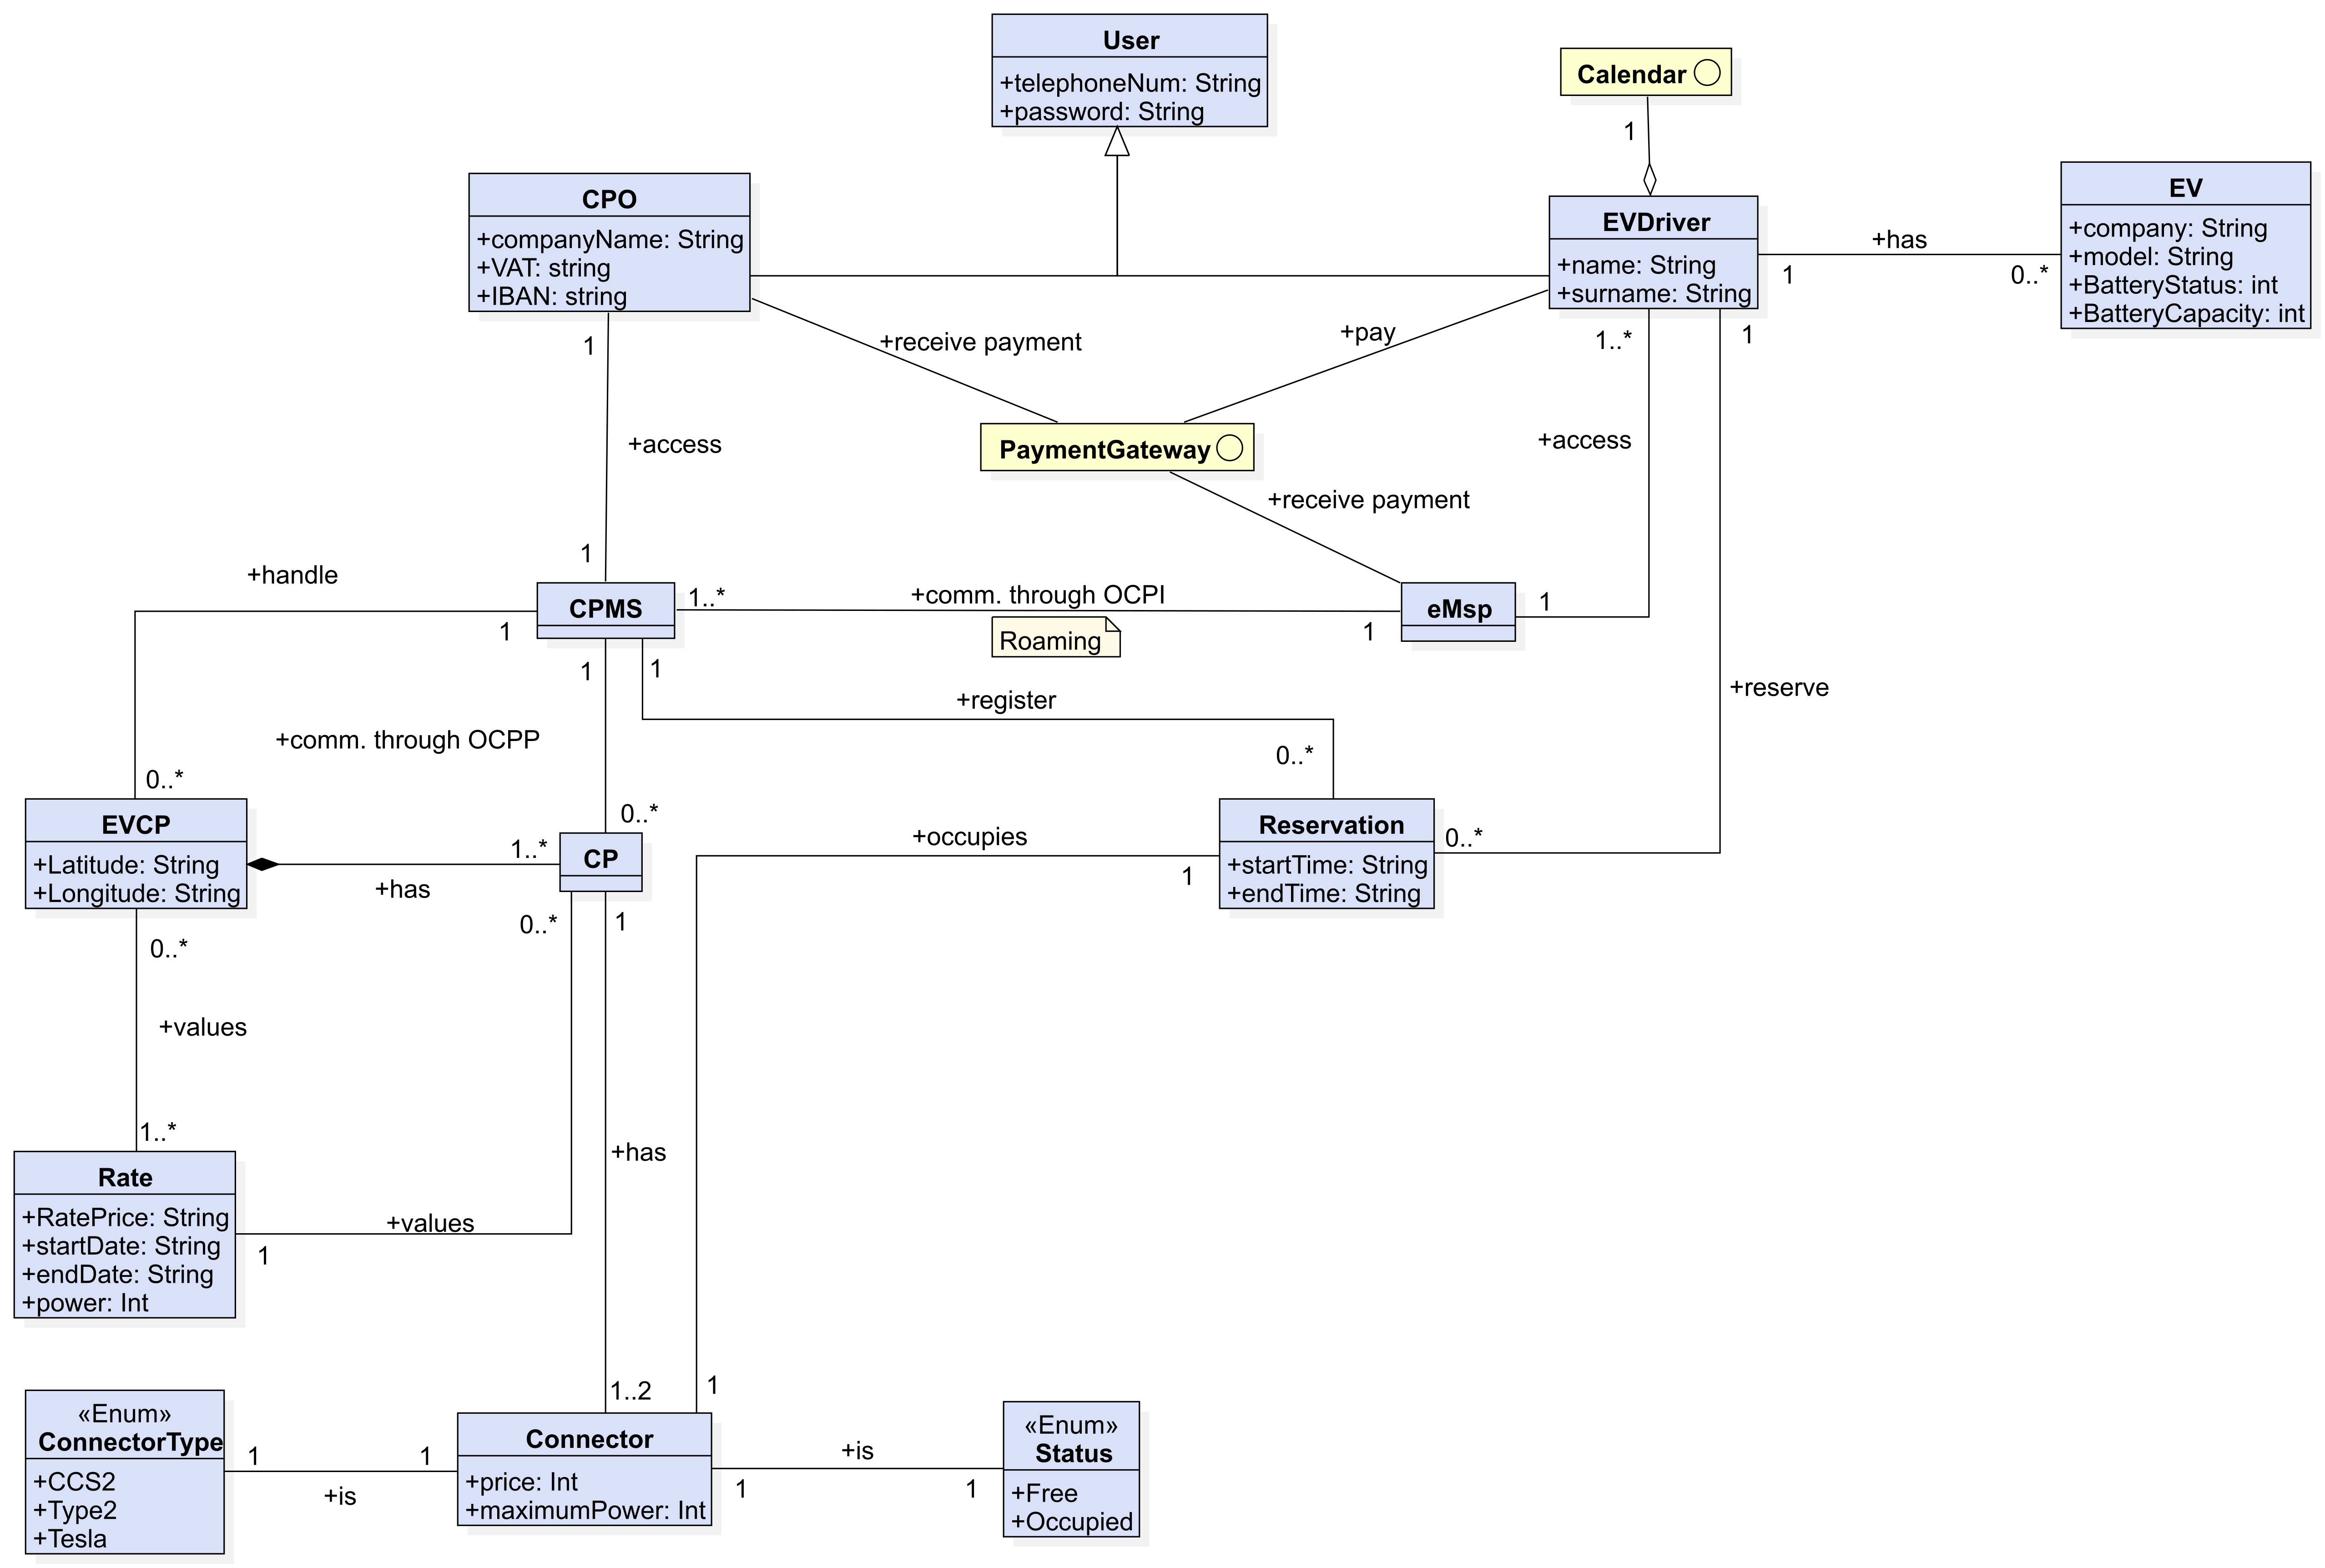
\includegraphics[scale=0.4]{src/domain_UML.png}
\end{figure} \vspace{1cm}

The main entity in the diagram are:
\begin{itemize}
      \item \textbf{User}\\
            A user can be a CPO or an EV Driver and their experience strictly depends on their role.
            An EV Driver has access to the eMsp entry point, while the CPOs access their CPMS.
            The EV Driver can pay for a charge through a Payment Gateway and the associated CPO receives the
            payment. Furthermore, EV Drivers can add their EVs to the system to receive a personalized experience and give the system access to their Calendar to receive suggestion based on their daily schedule
      \item \textbf{CPMS}\\
            The CPMS is a system that allows CPO to smartly handle their EVCPs. It provides automatically management of CPs but lets also the possibility to manually set options (the energy source mix, the DSO to acquire energy from ecc.). CPMSs communicate with eMsp following the OCPI protocol, this lets them being accessible from external eMsp too.
      \item \textbf{eMsp}\\
            The eMsp is the EV Driver entry point to the eMall system, it allows them to search for CPs, to book a connector for a given timeframe, pay and start a charge along with other functionalities described in the next chapters. The eMsp communicate with CPMSs following the OCPI protocol, this lets the EV drivers accessing CPs owned by CPO that aren't subscribed to our system and this leads to a larger set of possibilities
      \item \textbf{EVCP, CP, Connector}\\
            EVCP is a station with multiple CPs. Each CPs has usually 1 or 2 connectors that has a status and type. A CP communicates with CPMS following the OCPP protocol
\end{itemize}

\subsubsection{State diagrams}
In the paragraphs below, a representation of the behavior of the main conceptual
components of the system. The focus is on how these components respond to
external influences and modify accordingly their states. For this purpose, UML State Diagrams are proposed.\\
The following state diagram represents the possible status of a charging point.
When is added to the system it results "available" until the system requests to pass in "reserved" mode.
When it is in "reserved" status, only the user with the matching reservation can start a charge through the eMall APP.
When the user starts a charge the system communicates the charging point to change status in "charging". In this status
the charging point performs the charge as expected and when the charge is ended, the system notify to modify the status
in "available" back again. It is possible that for some sort of malfunction or manual intervention
by the operators through the system forces the charging point to change the status in "out of order", and this can happen from all the state. The charging point will return "available"
only when the operators decide to.
\begin{figure}[H]
      \centering
      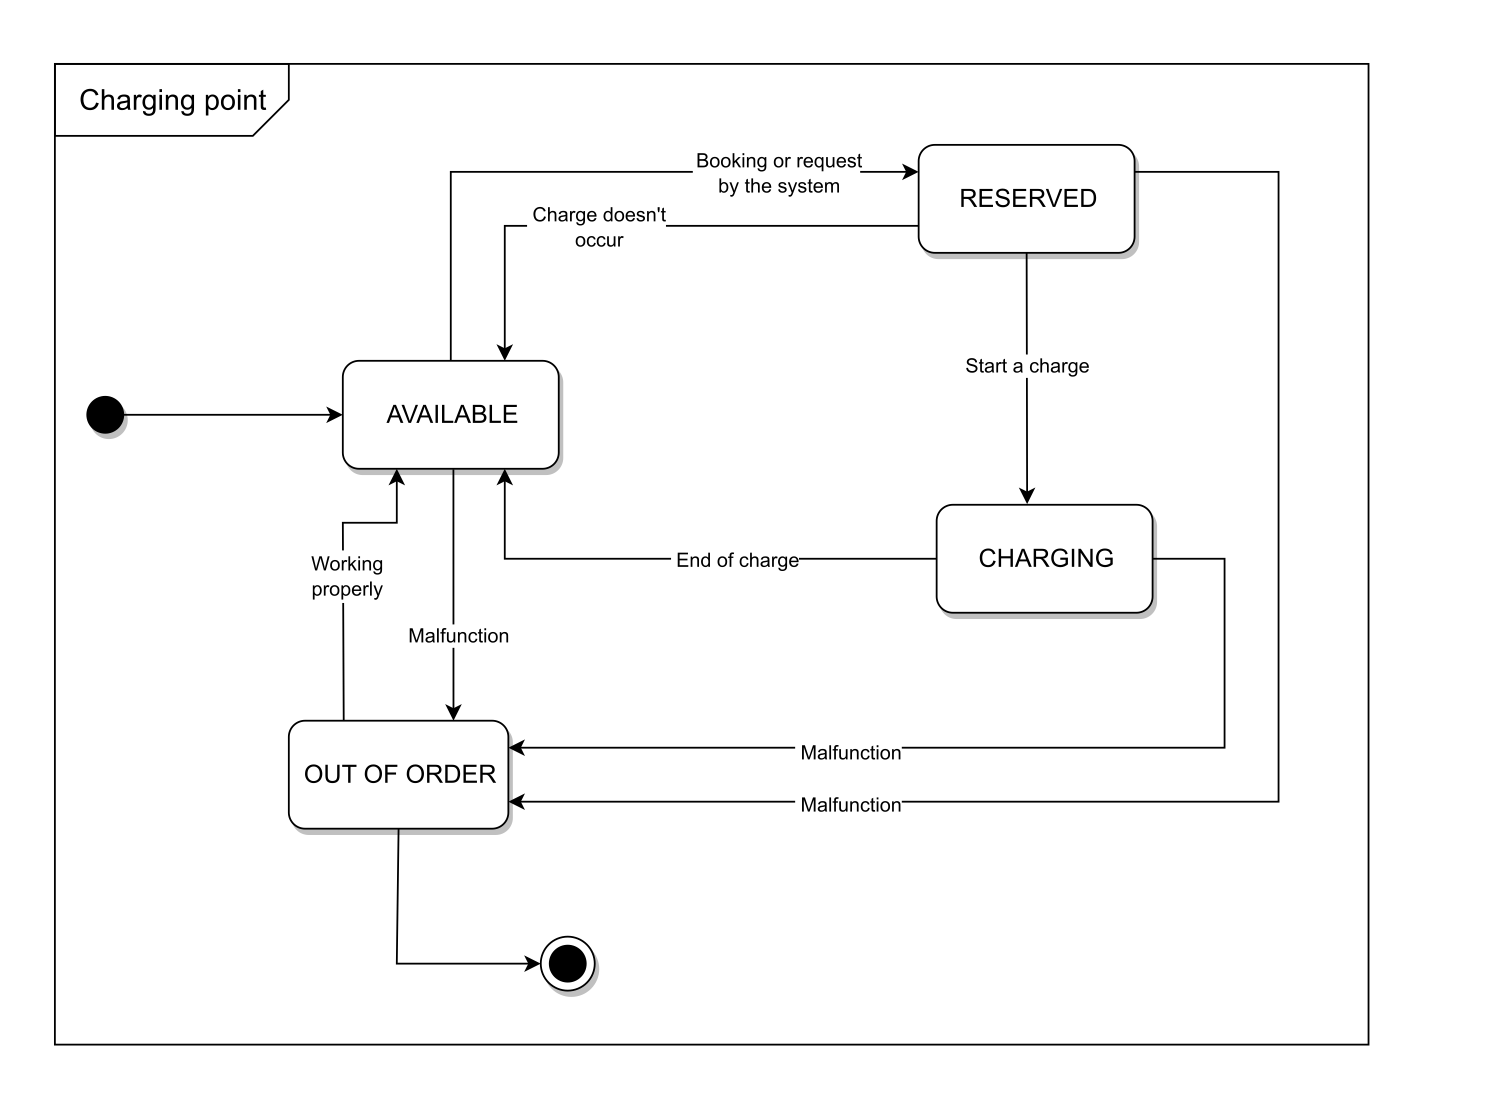
\includegraphics[scale=0.25]{src/state_diagram/cp.png}
      \caption{Charging Point state chart}
\end{figure} \vspace{1cm}


The following diagram describes the possible status for a reservation.
When a reservation is created through the APP it is in "not started" state. In the exact moment in which the time of the reservation starts
then it passes in the "pending" status. Will remain in pending status until the charge is started or until the time for the reservation runs out.
When the charge is started it is in "running" mode and when finishes is "completed" and archived in the list of past transaction.

\begin{figure}[H]
      \centering
      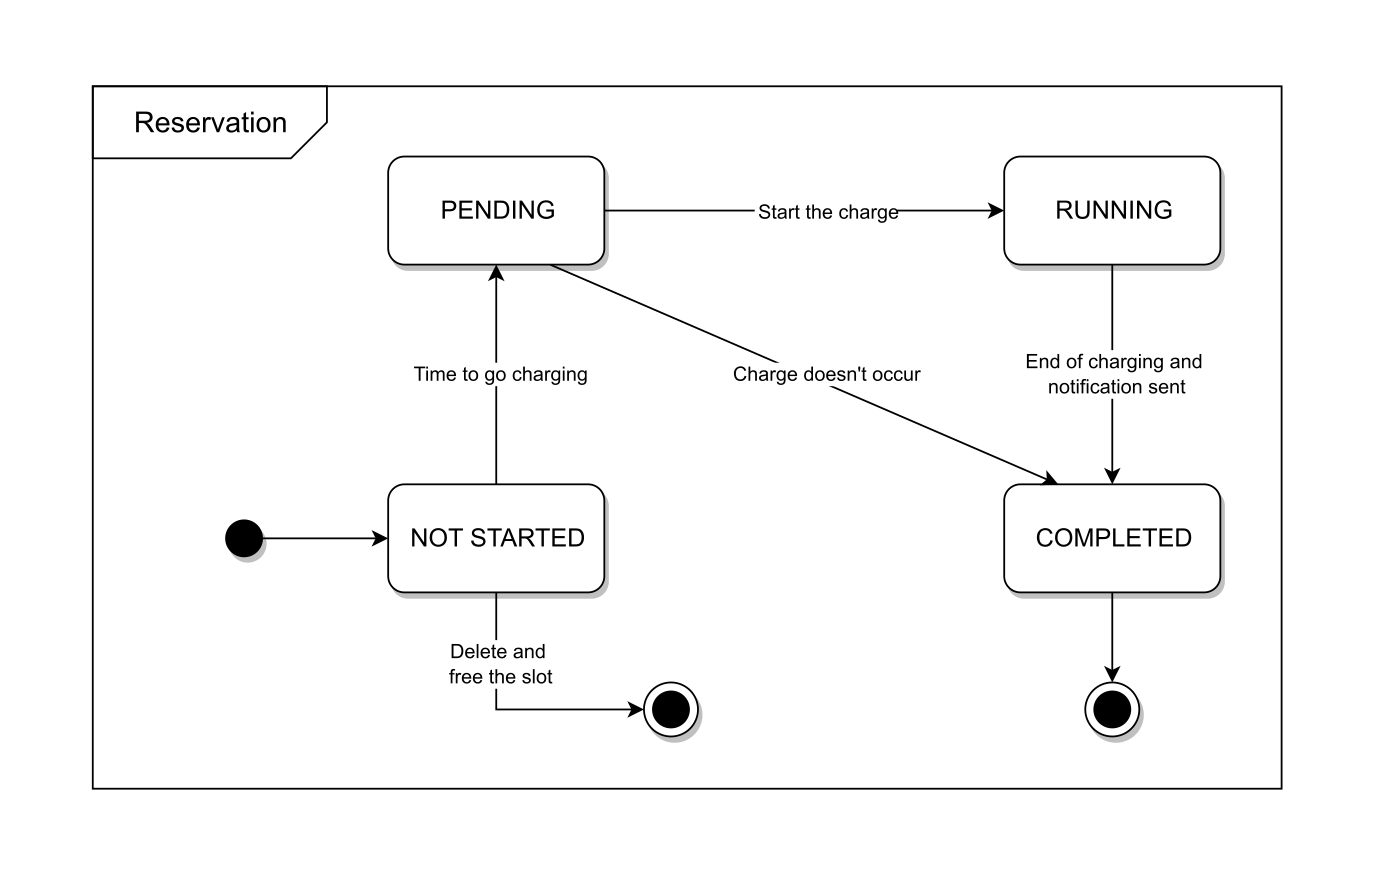
\includegraphics[scale=0.25]{src/state_diagram/transaction.png}
      \caption{Reservation state chart}
\end{figure} \vspace{1cm}

\subsection{Product functions}
The major functions offered by our system are organized according to the stakeholder that is being addressed
\begin{itemize}
      \item \textbf{EV driver's functions}\\
            The person that owns the EV to be smart charged. The function provided to the EV drivers aim to reduce the impact of charging processes on their daily schedule
            \begin{itemize}
                  \item \textbf{Search in Map}\\
                        Users can retrieve charging points based on some filtering, such as location, connectors available and booking date
                  \item \textbf{Receive smart charging suggestion}\\
                        Users receive suggestions on when and where to charge based on their location, the battery status of their EV, their daily schedule and special offer by CPOs
                  \item \textbf{Book a Charge}\\
                        Users can book a charge in a given charging point for a specified time frame and a chosen date. They can also pay through the system for the service
            \end{itemize}
\end{itemize}
\begin{itemize}
      \item \textbf{CPO's functions}\\
            The operator, person or entity, that manage the charging point at which the driver recharge their EV
            \begin{itemize}
                  \item \textbf{Monitor Status of CPs}\\
                        CPOs can retrieve the status of their CPs. The status contains the details about current charging processes, aggregate or detailed views of energy consumption, profit by each CP, and any problem reported by customers
                  \item \textbf{Manage DSOs contract}\\
                        CPOs can retrieve a list of available DSOs in their operating area, along with their energy prices. They can also create contract with DSOs and start getting energy from them
                  \item \textbf{Manually change status of a CP}\\
                        CPOs can manually reserve CPs or decide to set up a maintenance task, e.g. following a malfunction
                  \item \textbf{View reservations on their CPs}\\
                        CPOs can see a list of historical and live reservations on their CPs. The system provides them an aggregate or detailed view of reservations
                  \item \textbf{Managing CP}\\
                        CPOs can add, delete and modify CP. The system gives the possibility to make special offer, change prices and choose an energy sources mix
            \end{itemize}
\end{itemize}


\subsection{User characteristics}
It is possible to distinguish two different types of actors who use the system:
\begin{itemize}
      \item \textbf{EV driver}\\ People who want to book a charge remotely
            avoiding interference in their daily schedule, be notified when their reservations
            is going to start and end, monitor charging processes. Since there are not many statistical analyses on tech-friendliness among EV drivers, the system must aim to be usable by as wide an audience as possible providing easy to use interfaces
      \item \textbf{CPO}\\ People or entities who want to manage efficiently their EVCP, make statistics on live and historical details on the EVCP,
            to acquire information on the current price of energy offer by DSOs and to decide in an automated way
            where to get energy for charging. Operators are expert people who know details not known to drivers, know how to efficiently use a dashboard to modify and obtain the information they need
\end{itemize}


\subsection{Assumptions, dependencies and constraints}
\subsubsection{Domain Assumptions}
\begin{table}[H]
      \begin{tabularx}{\textwidth}{cX}
            \toprule
            \textbf{D1} & An EV driver arrives at the charging station at a time close to its reservation starting time \\
            \textbf{D2} & An EV driver leaves the charging station when the charge is finished                          \\
            \textbf{D3} & An EV driver doesn't occupy an already booked charging spot                                   \\
            \textbf{D4} & An EV driver provides correct information when registering                                    \\
            \textbf{D5} & At least one DSO can always provide energy to the CPOs                                        \\
            \textbf{D6} & An user that books a charge has an electric vehicle to charge                                 \\
            \textbf{D7} & An user that books a charge is always reliable                                                \\
            \bottomrule
      \end{tabularx}
\end{table}
\subsubsection{Dependencies}
\begin{table}[H]
      \begin{tabularx}{\textwidth}{cX}
            \toprule
            \textbf{Dep1}  & The system requires access to a third party maps API                                                           \\
            \textbf{Dep2}  & The system will use the GPS of the driver's computer or smartphone                                             \\
            \textbf{Dep3}  & The system will require internet connection to interact with all the users                                     \\
            \textbf{Dep4}  & The system will use an external API to retrieve the prices of energy by the available DSOs                     \\
            \textbf{Dep5}  & The system will use an external API to retrieve the EV battery status and a list of EV available on the market \\
            \textbf{Dep6}  & The system will use an external API to retrieve data or send data to the CPs                                   \\
            \textbf{Dep7}  & The system will use an external API to access the calendar of the users                                        \\
            \textbf{Dep8}  & The system will use a payment gateway to perform payment operations                                            \\
            \textbf{Dep9}  & The system will use an external API to send push notification to the drivers                                   \\
            \textbf{Dep10} & The system will use a third party API to send SMS to customers phones                                          \\
            \bottomrule
      \end{tabularx}
\end{table}
\subsubsection{Constraints}
\begin{itemize}
      \item The system shall be compliant to local laws and regulations, in particular users data should be treated
            according to the GDPR. This means that users should be always able to request their data
      \item The system should collect only necessary data, such as the user telephone number
      \item To better protect the users’ sensitive information, such as their telephone number and credentials, their data should be
            encrypted
      \item The external APIs, especially those critical for the correct functioning of the system, must be chosen among those with the highest availability and reliability
\end{itemize}